% @HEADER
% ***********************************************************************
% 
%            Trilinos: An Object-Oriented Solver Framework
%                 Copyright (2001) Sandia Corporation
% 
% Under terms of Contract DE-AC04-94AL85000, there is a non-exclusive
% license for use of this work by or on behalf of the U.S. Government.
% 
% This library is free software; you can redistribute it and/or modify
% it under the terms of the GNU Lesser General Public License as
% published by the Free Software Foundation; either version 2.1 of the
% License, or (at your option) any later version.
%  
% This library is distributed in the hope that it will be useful, but
% WITHOUT ANY WARRANTY; without even the implied warranty of
% MERCHANTABILITY or FITNESS FOR A PARTICULAR PURPOSE.  See the GNU
% Lesser General Public License for more details.
%  
% You should have received a copy of the GNU Lesser General Public
% License along with this library; if not, write to the Free Software
% Foundation, Inc., 59 Temple Place, Suite 330, Boston, MA 02111-1307
% USA
% Questions? Contact Michael A. Heroux (maherou@sandia.gov) 
% 
% ***********************************************************************
% @HEADER

\documentclass[11pt,relax]{SANDreport}
\usepackage{graphicx}
\usepackage{amsmath,amsfonts,amsthm}
\usepackage{amssymb}
\usepackage{enumerate}
\usepackage{rotating}


\usepackage{times}

\def\choicebox#1#2{\noindent$\hphantom{th}$\parbox[t]{1.8in}{\sf
#1}\parbox[t]{4.5in}{#2}\\[0.8em]}

\author{Michael Heroux and Marzio Sala \\
Computational Mathematics and Algorithms Department \\
Sandia National Laboratories \\
P.O. Box 5800 \\
Albuquerque, NM 87185-1110
}

\title{IFPACK 3.0 User's Guide}
\SANDnum{SAND2005-XXXX}
\SANDauthor{
Michael Heroux, Marzio Sala}

\SANDprintDate{January 2005}
\SANDreleaseType{Unlimited Release}

\newcommand{\Trilinos}{Trilinos}
\newcommand{\TrilinosTM}{Trilinos \copyright}
\newcommand{\trilinos}{{\sc Trilinos}}
\newcommand{\ifpack}{{\sc Ifpack}}
\newcommand{\aztecoo}{{\sc AztecOO}}
\newcommand{\amesos}{{\sc Amesos}}
\newcommand{\epetra}{{\sc Epetra}}
\newcommand{\ml}{{\sc ML}}
\newcommand{\mb}[1]{{\mathbf {#1} }}
\newcommand{\teuchos}{{\sc Teuchos}}
\newcommand{\triutils}{{\sc Triutils}}
\newcommand{\metis}{{\sc METIS}}

\newcommand{\ie}{i.e., }
\newtheorem{assumption}{Assumption}[section]
\newtheorem{lemma}{Lemma}[section]
\newtheorem{proposition}{Proposition}[section]
\newtheorem{corollary}{Corollary}[section]
\newtheorem{theorem}{Theorem}[section]
\newtheorem{algorithm}{Algorithm}[section]
\newtheorem{definition}{Definition}[section]
\newtheorem{property}{Property}[section]

\newtheorem{remark}{Remark}

\def\choicebox#1#2{\noindent$\hphantom{th}$\parbox[t]{3.0in}{\sf
#1}\parbox[t]{3.35in}{#2}\\[0.8em]}

\begin{document}

\maketitle

\begin{abstract}
\ifpack~provides a suite of object-oriented algebraic preconditioners
for the solution of preconditioned iterative solvers.  \ifpack~constructors 
expect the (distributed) real sparse matrix to be an Epetra\_RowMatrix object.
\ifpack~, as part of the Trilinos Solver Project,
interacts well with other Trilinos packages. In particular, \ifpack~objects
can be used as preconditioners for \aztecoo, and as smoothers for \ml. 

\ifpack\ can be used to define point and block relaxation preconditioners,
  various flavors of incomplete factorizations for symmetric and non-symmetric
  matrices, and one-level additive Schwarz preconditioners with variable
  overlap. Exact LU factorizations can be accessed through the \amesos\
  packages.

\ifpack\ is mainly written in C++, but only  a limited subset of C++ features
is used, in order to enhance portability.
\end{abstract}

\clearpage
\section*{Acknowledgments}
The authors would like to acknowledge the support of the ASCI and LDRD programs
that funded development of Trilinos.

\medskip

\SANDmain

\tableofcontents

\clearpage
\newpage
% HEADER
% ***********************************************************************
% 
%            Trilinos: An Object-Oriented Solver Framework
%                 Copyright (2001) Sandia Corporation
% 
% Under terms of Contract DE-AC04-94AL85000, there is a non-exclusive
% license for use of this work by or on behalf of the U.S. Government.
% 
% This library is free software; you can redistribute it and/or modify
% it under the terms of the GNU Lesser General Public License as
% published by the Free Software Foundation; either version 2.1 of the
% License, or (at your option) any later version.
%  
% This library is distributed in the hope that it will be useful, but
% WITHOUT ANY WARRANTY; without even the implied warranty of
% MERCHANTABILITY or FITNESS FOR A PARTICULAR PURPOSE.  See the GNU
% Lesser General Public License for more details.
%  
% You should have received a copy of the GNU Lesser General Public
% License along with this library; if not, write to the Free Software
% Foundation, Inc., 59 Temple Place, Suite 330, Boston, MA 02111-1307
% USA
% Questions? Contact Michael A. Heroux (maherou@sandia.gov) 
% 
% ***********************************************************************
% @HEADER

%-----------------------------------------------------------------------------
\section{Introduction}
\label{chap:introduction}
%-----------------------------------------------------------------------------

The parallel solution of large linear systems of type
\begin{equation}
\label{eq:linear_sys}
A {x} = {b},
\end{equation}
where $A$ is a (distributed) large, sparse matrix and $x$ and $b$ two real
multi-vectors, is often achieved using iterative solvers of Krylov type (see for
instance~\cite{barret93templates}).
It is well known that the convergence of Krylov methods depends on 
the spectral properties of the linear system matrix
$A$~\cite{axelsson94iterative,saad96iterative,QSS}. Hence, the
original system~(\ref{eq:linear_sys}) is often replaced by
\[
P^{-1} A{u} = P^{-1} {b}
\]
(left-preconditioning), or by
\[
A P^{-1} P {u} = {b}
\]
(right-preconditioning), using a linear transformation $P^{-1}$,
called {\sl preconditioner}, in order to improve the spectral properties of
the linear system matrix. In general terms, a preconditioner is any
kind of transformation applied to the original system which makes it
easier to solve, in terms of iterations and CPU time.

The general (and challenging) problem of finding an efficient
preconditioner is to identify a linear operator $P$ with the following
properties:
\begin{enumerate}
\item {\bf $P$ is a good approximation of $A$ is some sense}. Although no
  general theory is available, we can say that $P$ should act so that
  $P^{-1} A$ is near to being the identity matrix and its eigenvalues
  are clustered within a sufficiently small region of the complex plane 
  (see for instance~\cite{greenbaum97iterative});
\item {\bf $P$ is efficient}, in the sense that the iteration method converges
  much faster, in terms of CPU time, for the preconditioned system.  In
  other words, preconditioners must be selected in such a way that the
  cost of constructing and using them is offset by the improved
  convergence properties they permit to achieve;
\item {\bf $P$ or $P^{-1}$ can be constructed in parallel}, to take advantage of the architecture of modern supercomputers.
\end{enumerate}

The choice of $P$ varies from ``black-box'' algebraic techniques which
can be applied to general matrices to ``problem dependent''
preconditioners which exploit special features of a particular class
of problems. Although problem dependent preconditioners can be very
powerful, there is still a practical need for efficient
preconditioning techniques for large classes of problems. \ifpack\ aims to
fill the need for general, black-box preconditioners, by providing a set of
robust algebraic preconditioners for parallel large scale applications.

Single-level algebraic preconditioners can be classified as follows:
\begin{enumerate}
\item {\bf Relaxation schemes},
  like Jacobi, Gauss-Seidel and symmetric Gauss-Seidel (point or block versions)~\cite{varga00matrix}.
  These schemes seldomly provide satisfactory performances as stand-alone
  preconditioner, but can be very effective if used as smoothers in
  multilevel methods (like, for example, ML~\cite{ml-guide});
\item {\bf Polynomial preconditioner}, like Neumann, Least-Square, and
Chebyshev~\cite{saad96iterative}.
\item {\bf Incomplete Factorizations preconditioner}, like ILU(k), RILU(k);
\item {\bf One-level domain decomposition preconditioners of Schwarz type},
  with minimal or wider overlap among the subdomains~\cite{smith96parallel,
    QV2}. The local linear problems
  can be solved with exact factorizations, incomplete factorizations, or
  {\sl any} other \ifpack\ preconditioner documented in this manual. 
  For example, each subdomain matrix
  can be furtherly decomposed into subdomains, and block preconditioner can be
  applied to solve the local problem. 
\item {\bf Sparse Approximate Inverses} (like SPAI, AINV).
\end{enumerate}
\ifpack\ aims to define preconditioners belonging to groups 1, 3 and 4.
Preconditioners of class 2 can be accessed through AztecOO. Libraries like
ParaSails or SPAI are available to define preconditioners of class 5 
(see for instance~\cite{grote97parallel,benzi98sparse}).

\begin{remark}
Single-level preconditioners can be used as stand-alone preconditioners, on in
conjunction with multilevel preconditioners. In this latter case, the
single-level preconditioner is reinterpreted as a smoother for the multilevel
hierarchy. Two families of methods have been
proposed in the literature:
the classical Ruge-Stuben multigrid (AMG), or smoothed aggregation (SA).
The preconditioning package Hypre can be used to define AMG preconditioners,
  while the Trilinos package ML can be used to build SA preconditioners.
\end{remark}

\smallskip

The goal of this document is to provide an overview of all \ifpack\
  preconditioners. Several examples are reported to illustrate how to define
  and use \ifpack\ objects. Further details can be found on the Doxygen
  documentation.
The manuscript is organized as follows. Section\ref{sec:theo} briefly outlines
the theoretical background. A general description of \ifpack\
  preconditioners is reported in Section~\ref{sec:prec}.
Parameters for \ifpack~preconditioners are reported in
Section~\ref{sec:parameters}. The \ifpack\ factory class is detailed in
Section~\ref{sec:factory}. Several examples of usage are reported in
Section~\ref{sec:usage}. The analysis tools of \ifpack\ are reported in
Section~\ref{sec:analysis}. Configuration and building are detailed in
Section~\ref{sec:config}.

%-----------------------------------------------------------------------------
\section{Theoretical background}
\label{sec:theo}
%-----------------------------------------------------------------------------

The aim of this section is to define concepts associated with algebraic
preconditioning and establish our notation. This section is not
supposed to be exhaustive, nor complete on this subject. The reader is
referred to the existing literature for a comprehensive presentation.

\medskip

%-----------------------------------------------------------------------------
\subsection{Point Preconditioners}
\label{sec:point}
%-----------------------------------------------------------------------------

\ifpack\ contains a set of simple point preconditioners based on relaxation
methods.
Beginning with a given approximate solution, these methods modify the
components of the approximation, one or a few at a time and in a certain order,
until convergence is reached. Although still popular in some application
areas, these preconditioners are now
rarely used; however, they can provide successful smoothers for multilevel
methods. 

All \ifpack\ point preconditioners are based on the decomposition
\begin{equation}
\label{eq:splitting}
A = D - E - F,
\end{equation}
where $D$ is the diagonal part of $A$, $-E$ the strict lower part, and 
$-F$ the strict upper part. It is always assumed that the diagonal entries of
$A$ are all nonzero.

%-----------------------------------------------------------------------------
\subsubsection{Point Jacobi Preconditioner}
\label{sec:jacobi}
%-----------------------------------------------------------------------------

Given a starting solution $x^{(0)}$, the (damped) Jacobi method determines 
the $i-$th component of 
solution of (\ref{eq:linear_sys}) at step $k \geq 1$ as
\[
a_{i,i} x^{(k)}_i = \omega \; \left[  \;- \sum_{j \neq i} a_{i,j} x^{(k-1)} + b_i
\; \right]
\]
where $\omega$ is the damping parameter\footnote{Clearly, is used as a
  solver, $\omega$ must be set to 1 to converge to the solution of
    (\ref{eq:linear_sys}).} and
$a_{i,j}$ the $(i,j)$ element of matrix $A$.
This component-wise equation can be rewritten in a vector form as
\[
x^{(k)} = \omega \; \left[ \; D^{-1} (E+F) x ^{(k-1)} + D^{-1} b \; \right],
\]
or, equivalently,
\begin{equation}
\label{eq:jacobi}
x^{(k)} = x^{(k-1)} + \omega D^{-1} (b - A x ^{(k-1)} ) =
          x^{(k-1)} + \omega D^{-1} r^{(k-1)},
\end{equation}
where $r^{(k-1)} = b - A x ^{(k-1)}$ is the residual at step $k-1$. 

This preconditioner is symmetric.

%-----------------------------------------------------------------------------
\subsubsection{Point Gauss-Seidel Preconditioner}
\label{sec:gs}
%-----------------------------------------------------------------------------

The (damped) Gauss-Seidel method at step $k \geq 1$ can be written as
\[
a_{i,i} x^{(k)}_i = \omega \; 
 \left[- \sum_{j<i} a_{i,j} x^{(k)} 
			   - \sum_{j>i} a_{i,j} x^{(k-1)} + b_i
			   \; \right]
\]
where $\omega$ is the damping parameter. In vector form, one has
\begin{equation}
\label{eq:gs}
x^{(k)} = x^{(k-1)} + \omega (D - E)^{-1} (b - A x ^{(k-1)} ) ,
\end{equation}
which requires, at each step $k$, the solution of a (lower) triangular 
linear system. This preconditioner is non-symmetric.

%-----------------------------------------------------------------------------
\subsubsection{Point SOR Preconditioner}
\label{sec:sor}
%-----------------------------------------------------------------------------

The Successive Over Relaxation (SOR) method computes the $k$-th step 
using the relaxation sequence
\begin{equation}
\label{eq:sor}
x^{(k)} = \omega x_{GS}^{(k-1)} + (1 - \omega) x^{(k-1)}, 
\end{equation}
where $x_{GS}^{(k-1)}$ is the $k-1$ step of a (non-damped) Gauss-Seidel
iteration. SOR is based on the splitting 
\[
\omega A = (D - \omega E) - (\omega F + (1 - \omega) D ) ,
\]
so that (\ref{eq:sor}) can also be written as
\[
(D - \omega E) x^{(k)} = \left[
\omega F + (1 - \omega ) D
\right] x^{(k-1)} + \omega b.
\]
This preconditioner is non-symmetric.

%-----------------------------------------------------------------------------
\subsubsection{Point SSOR Preconditioner}
\label{sec:ssor}
%-----------------------------------------------------------------------------

A Symmetric SOR (SSOR) step consist of the SOR step (\ref{eq:sor}) followed by
a backward SOR,
\begin{equation}
\label{eq:ssor}
\begin{array}{rcl}
(D - \omega E) x^{(k-1/2)} &= &[ \omega F - (1 - \omega)D] x^{(k-1)} + \omega b \\
(D - \omega F) x^{(k)} &=& [ \omega E - (1 - \omega)D] x^{(k-1/2)} + \omega b .
\end{array}
\end{equation}
This preconditioner is symmetric. When $\omega = 1$, we obtain
\begin{equation}
\label{eq:sgs}
\begin{array}{rcl}
(D - E) x^{(k-1/2)} &= & F x^{(k-1)} + b \\
(D - F) x^{(k)}     &= & E  x^{(k-1/2)} + b .
\end{array}
\end{equation}
This method
is often called symmetric Gauss-Seidel.

%-----------------------------------------------------------------------------
\subsection{Block Preconditioners}
\label{sec:block}
%-----------------------------------------------------------------------------

Block preconditioners of Jacobi and Gauss-Seidel type generalize their point
counterpart by updating a set of variables at the same time. Consider
to partition the matrix $A$, the right-hand side and the solution vector
as follows:
\begin{equation}
\label{eq:partition}
A = 
\left(
\begin{array}{c c c c c}
A_{1,1} & A_{1,2} & A_{1,3} & \ldots & A_{1,m} \\
A_{2,1} & A_{2,2} & A_{2,3} & \ldots & A_{2,m} \\
A_{3,1} & A_{3,2} & A_{3,3} & \ldots & A_{3,m} \\
\vdots  & \vdots  & \vdots  & \ddots & \vdots  \\
A_{m,1} & A_{m,2} & A_{m,3} & \ldots & A_{m,m} \\
\end{array}
\right),
  \;\;\;
x = 
\left(
\begin{array}{c c c c c}
x_{1} \\
x_{2} \\
x_{3} \\
\vdots  \\
x_{m}
\end{array}
\right), \;\;\;
b = 
\left(
\begin{array}{c c c c c}
b_{1} \\
b_{2} \\
b_{3} \\
\vdots  \\
b_{m}
\end{array}
\right),
\end{equation}
in which the partitioning of $x$ and $b$ into $m$ blocks is compatible with the partitioning
of $A$. Also, it is supposed that the diagonal blocks $A_{i,i}$ are square
and assumed nonsingular.

Splitting (\ref{eq:splitting}) can still be used to define block Jacobi
and block Gauss-Seidel algorithms, with the following definitions of $D$, $E$
and $F$:
\begin{equation}
\label{eq:D}
D = 
\left(
\begin{array}{c c c c c}
A_{1,1} &         &         &        &          \\
        & A_{2,2} &         &        &          \\
        &         & A_{3,3} &        &          \\
        &         &         & \ddots &         \\
        &         &         &        & A_{m,m} \\
\end{array}
\right), 
\end{equation}
\begin{equation}
\label{eq:E}
E =  -
\left(
\begin{array}{c c c c c}
 O      &         &         &        &          \\
A_{2,1} & O       &         &        &          \\
A_{3,1} & A_{3,2} & O       &        &          \\
 \vdots & \vdots  &         & \ddots &         \\
A_{m,1} & A_{m,2} & A_{m,3} & \ldots &     O    \\
\end{array}
\right), 
\end{equation}
\begin{equation}
\label{eq:F}
F =  -
\left(
\begin{array}{c c c c c}
 O      & A_{1,2} & A_{1,3} & \ldots & A_{1,m}  \\
        & O       & A_{2,3} & \ldots & A_{2,m}  \\
        &         & O       &        &          \\
        &         &         & \ddots &         \\
        &         &         &        &     O    \\
\end{array}
\right), 
\end{equation}

Using definitions (\ref{eq:D}), (\ref{eq:E}) and (\ref{eq:F}), the block
Jacobi method is simply as reported in equation (\ref{eq:jacobi}). Analogously,
the block Gauss-Seidel is still described by equation (\ref{eq:gs}), and
the symmetric Gauss-Seidel by equation (\ref{eq:sgs}).

Let us suppose to partition the set of rows of 
the matrix into $m$ sets $S_i, i=1, \ldots,m$, such that
\[
S_i \subseteq S, \quad \cup_i S_i = S.
\]
Let $V_i$ be a
boolean $n \times n_i$ matrix (where $n_i = card(S_i)$), whose entries are
defined as
\[
V_{i,j} = \left\{
\begin{array}{l l}
1 & \mbox{ if } i \in S_j \\
  0 & \mbox{otherwise}
\end{array}
  \right.
\]
A general (damped) block Jacobi iteration can be defined as follows:
\begin{eqnarray}
&& \mbox{On each processor, for each block $i$, Do} \\
&& \label{eq:gen_b_jacobi}
x^{(k)} = x^{(k-1)} + \omega V_i^T A_{i,i}^{-1} V_i(b - A x^{(k-1)}).
\end{eqnarray}
In Equation (\ref{eq:gen_b_jacobi}), it is understood that the $x$ vectors
refer to the local components.
Figure~\ref{fig:bj} graphically describes the block Jacobi with variable
overlap among blocks.

\begin{figure}
\begin{center}
\includegraphics[width=6cm]{bj.eps}
\end{center}
\caption{The block Jacobi matrix with overlapping blocks.}
\label{fig:bj}
\end{figure}

The (damped) block Gauss-Seidel algorithm easily derives from
(\ref{eq:gen_b_jacobi}), by immediately updating the solution vector to
compute the residual. The algorithm is as follows:
\begin{eqnarray}
&& \mbox{On each processor, for each block $i$, Do} \\
&& \label{eq:gen_b_gs}
x^{(k)} = x^{(k-1)} + \omega V_i^T A_{i,i}^{-1} V_i(b - A x^{(k)}).
\end{eqnarray}

%-----------------------------------------------------------------------------
\subsection{Additive Schwarz Preconditioners}
\label{sec:additive}
%-----------------------------------------------------------------------------

\ifpack\ makes very easy to define and use domain decomposition
preconditioners of (overlapping) Schwarz type.

The basic idea of DD methods is to decompose the
computational domain $\Omega$ into $M$ smaller parts $\Omega_i$,
$i=1,\ldots,M$, called subdomains, such that $\cup_{i=1}^{M}
\overline{\Omega_i} = \overline{\Omega}$.  Next, the original problem can
be reformulated within each subdomain $\Omega_i$, of smaller size. This
family of subproblems is coupled one to another through the values of the
unknown solution at subdomain interface. This coupling is then removed at
the expense of introducing an iterative process which involves, at each
step, solutions on the $\Omega_i$ with additional interface conditions on
$\partial \Omega_i \setminus \partial \Omega$.

In overlapping Schwarz preconditioner, the computational domain is
subdivided into {\sl overlapping} subdomains, and local Dirichlet-type
problems are then solved on each subdomain.  The communication between the
solutions on the different subdomains is here guaranteed by the overlapping
region. 

The additive Schwarz preconditioner can be written as:
\begin{equation}
\label{eq:as}
P_{AS}^{-1} = \sum_{i=1}^M P_i A_i^{-1} R_i ,
\end{equation}
where $M$ is the number of subdomains (that is, the number of processors in
the computation), $R_i$ is an operator that restricts the global 
vector to the vector lying on subdomain $\Omega_i$, $P_i$ is an operator that
prolongate from subdomain $\Omega_i$ to $\Omega$, and
\begin{equation}
\label{eq:Ai}
A_i = R_i A P_i.
\end{equation}

\ifpack\ supports two major cases:
\begin{itemize}
\item Minimal-overlap (here referred to as "zero-overlap"): each subdomain
is identified by the set of local rows of the preconditioned matrix;
\item General overlap: each subdomain is identified by the set of local rows
of a suitable overlapping matrix.
\end{itemize}
In both cases, each processor is responsible for exactly one subdomain.

In the minimal overlap case, the $R_i$'s and $P_i$'s are not implemented, since the
required components of the residual vector are already local. Besides, matrix
(\ref{eq:Ai}) can be easily extracted from the local matrix, by dropping all
nonzeros corresponding to non-local columns.
communications between processors. If a wider overlap
is used, instead, each application of $R_i$ and $P_i$ may require the
importing or exporting of
off-process data, and the construction of (\ref{eq:Ai}) requires
communications.

\smallskip

Once matrices (\ref{eq:Ai}) have been formed, the user still need to define a
strategy to apply the inverse of $A_i$ in (\ref{eq:as}). At this purpose,
any \ifpack\ preconditioner can be adopted. Common choices can be:
\begin{itemize}
\item To solve exactly on each subdomain with an complete LU factorization, using the \verb!Ifpack_Amesos!
preconditioner. This is shown in Section~\ref{sec:as_amesos}.
\item To solve using an incomplete LU factorization, as presented in
Section~\ref{sec:as_ilu}.
\item To furtherly decompose the local domain into smaller subdomains,
  then apply a block Jacobi or block Gauss-Seidel preconditioner. This is
  outlined in Section~\ref{sec:as_b_ov}.
\end{itemize}

\begin{remark}
Additive Schwarz preconditioners as reported in equation~(\ref{eq:as}) 
are not scalable: their convergence rate
deteriorates as the number of subdomains (that is, of the processors)
increases. Algebraic techniques
exist to add an algebraic coarse level correction to~(\ref{eq:as}) to make the
preconditioner scalable; 
see for example the documentation of the ML
package~\cite{ml-guide}.
\end{remark}

%-----------------------------------------------------------------------------
\subsection{Incomplete Factorization Preconditioners}
\label{sec:ilu}
%-----------------------------------------------------------------------------

A broad class of effective preconditioners is based on incomplete
factorization of the linear system matrix.  Such preconditioners are often
referred to as incomplete lower/upper (ILU) preconditioners.  
ILU preconditioning techniques lie between direct and
iterative methods and provide a balance between reliability and
numerical efficiency.  ILU preconditioners are constructed in the factored form
$P=\tilde{L} \tilde{U}$, with $\tilde{L}$ and $\tilde{U}$ being lower
and upper triangular matrices. Solving with $P$ involves two triangular
solutions.

ILU preconditioners are based on the observation
that, although most matrices $A$ admit an LU factorization $A=LU$, where $L$ is
(unit) lower triangular and $U$ is upper triangular, the factors $L$ and $U$ often
contain too many nonzero terms, making the cost of factorization too expensive in
time or memory use, or both.  One type of ILU preconditioner is ILU(0), which 
is defined as proceeding through the standard LU decomposition computations, but keeping 
only those terms in $\tilde{L}$ that correspond to nonzero terms in the lower
triangle of $A$ and similarly keeping only those terms in $\tilde{U}$ that 
correspond to nonzero terms in the upper triangle of $A$.  Although effective, in
some cases the accuracy of the ILU(0) may be insufficient to yield an
adequate rate of convergence. More accurate factorizations will differ
from ILU(0) by allowing some {\em fill-in}. The resulting class of
methods is called ILU($k$), where $k$ is the level-of-fill. A
level-of-fill is attributed to each element that is processed by
Gaussian elimination, and dropping will be based on the level-of-fill.
The level-of-fill should be indicative of the size of the element: the
higher the level-of-fill, the smaller the elements.  

Other strategies consider dropping by value -- for example, dropping
entries smaller than a prescribed threshold. Alternative dropping
techniques can be based on the numerical size of the element to be
discarded. Numerical dropping strategies generally yield more accurate
factorizations with the same amount of fill-in as level-of-fill
methods. The general strategy is to compute an entire row of the
$\tilde{L}$ and $\tilde{U}$ matrices, and then keep only a certain
number of the largest
entries. In this way, the amount of fill-in is
controlled; however, the structure of the resulting matrices is
undefined. These factorizations are usually referred to as ILUT($k$).

When solving a single linear system, ILUT($k$) methods can be more effective
than ILU($k$).  However, in many situations a sequence of linear systems
must be solved where the pattern of the matrix $A$ in each system is
identical but the values of changed.  In these situations, ILU($k$) is 
typically much more effective because the pattern of ILU($k$) will also
be the same for each linear system and the overhead of computing the
pattern is amortized.

%-----------------------------------------------------------------------------
\section{General Description of \ifpack\ Preconditioners}
\label{sec:prec}
%-----------------------------------------------------------------------------

All \ifpack\ preconditioners described in this document
are reported in Table~\ref{tab:all_prec}. They are all derived from the 
\verb!Ifpack_Preconditioner.h!
class.

%\begin{figure}
%\begin{center}
%\includegraphics[width=15cm]{Ifpack_Preconditioner.eps}
%\caption{FIXME: UML diagram of  several \ifpack\ preconditioners.}
%\label{fig:if_prec}
%\end{center}
%\end{figure}

\begin{sidewaystable}
\begin{center}
\begin{tabular}{|p{6cm} | c |p{12cm} |}
\hline
Class name & Overlap & Description \\
\hline
\hline
\verb!Ifpack_PointRelaxation!   & 0 & Point (damped) relaxation
preconditioners (Jacobi, Gauss-Seidel, symmetric Gauss-Seidel). Users
can specify the number of Jacobi steps (sweeps), and the damping factor. See
Section~\ref{sec:jacobi} \\
\hline
\verb!Ifpack_BlockRelaxation! & 0 & Block relaxation
preconditioner (Jacobi, Gauss-Seidel, symmetric Gauss-Seidel). Users can store the diagonal blocks as dense or sparse. In the
latter case, any \ifpack\ preconditioner can be used to apply the inverse of
the diagonal block. See Section~\ref{sec:block}. \\
\hline
\verb!Ifpack_AdditiveSchwarz! & user & Generic additive Schwarz
preconditioner. Allows for generic additive Schwarz preconditioners, with
minimal or wider overlap. In the latter case, the user must provide
the overlapping matrix. Any \ifpack\ preconditioner can be used to
solve the local problems. See Section~\ref{sec:additive}. \\
\hline
\verb!Ifpack_IC! & 0 & Incomplete Cholesky factorization, with dropping based
on the level-of-fill of the graph. \\
\hline
\verb!Ifpack_ICT! & 0 & Incomplete Cholesky factorization, with dropping based
on threshold.\\
\hline
\verb!Ifpack_ILU! & 0 & Incomplete LU factorization, with dropping based
on the level-of-fill of the graph. \\
\hline
\verb!Ifpack_ILUT! & 0 & Incomplete LU factorization, with dropping based
on threshold. \\
\hline
\hline
\end{tabular}
\caption{Description of all the \ifpack\ preconditioners reported in this
  document. In the Table, `Overlap' indicates the overlap (with 0 being the
  minimal overlap case, `any' means that the code can construct the
  overlapping matrix for any given positive value).}
\label{tab:all_prec}
\end{center}
\end{sidewaystable}

\verb!Ifpack_Preconditioner.h! is a pure virtual class, derived from
\verb!Epetra_Operator!, that standarizes the construction of \ifpack\
preconditioners. In fact, all \ifpack\ preconditioners are supposed to behave
as follows:
\begin{enumerate}
\item The object is constructed, passing as only input argument the
pointer of the matrix to be preconditioned, say {\tt A}. {\tt A} has already
been {\tt FillComplete()}'d.
%
\item All the parameters, stored in a \teuchos\ parameters list, are
set using method \verb!SetParameters()!. If \verb!SetParameters()! is not
called, default values will be used.
%
\item The preconditioner is initialized by calling method \verb!Initialize()!.
In this phase, all operations that do not require the matrix values of {\tt A}
are performed (that is, only the structure of {\tt A} is used).
%
\item The preconditioner is constructed by calling method \verb!Compute()!.
In this phase, all the operations that require the matrix values of {\tt A}
are performed
\footnote{For example, in a time dependent setting, if the structure of {\tt
  A} does not change from a given time step to the next but its values do,
  the user can call {\tt Initialize()} only once before the first time step,
  then {\tt Compute()} at each time step.}.
%
\item Method \verb!ApplyInverse()! applies the preconditioner. Any class that
uses \verb!ApplyInverse()! to apply the preconditioner can take advantage of
an \verb!Ifpack_Preconditioner! derived object\footnote{For example, {\tt
  AztecOO} objects can use {\tt Ifpack\_Preconditioner} objects as
    preconditioners.}.
%
\item Method \verb!IsInitialized()! returns {\tt true} is the preconditioner has
been successfully initialized, {\tt false} otherwise.
%
\item Method \verb!IsComputed()! returns {\tt true} is the preconditioner has
been successfully computed, {\tt false} otherwise.
%
\item Method \verb!Condest()! returns an estimation of the condition
number of the preconditioned system.
The condition of a matrix $B$, called $cond_p(B)$, is defined as
$cond_p(B) = \|B\|_p\|B^{-1}\|_p$ in some appropriate norm $p$. 
$cond_p(B)$
gives some indication of how many accurate floating point
digits can be expected from operations involving the matrix and its
inverse.  A condition number approaching the accuracy of a given
floating point number system, about 15 decimal digits in IEEE double
precision, means that any results involving $B$ or $B^{-1}$ may be
meaningless.

The $\infty$-norm of a vector $y$ is defined as the maximum of the
absolute values of the vector entries, and the $\infty$-norm of a
matrix C is defined as
$\|C\|_\infty = \max_{\|y\|_\infty = 1} \|Cy\|_\infty$.
A crude lower bound for the $cond_\infty(C)$ is
$\|C^{-1}e\|_\infty$ where $e = (1, 1, \ldots, 1)^T$.  It is a
lower bound because $cond_\infty(C) = \|C\|_\infty\|C^{-1}\|_\infty
\ge \|C^{-1}\|_\infty \ge |C^{-1}e\|_\infty$. 

More accurate (and expensive) computations for the condition number can be
obtained by calling {\tt Condest(Ifpack\_CG)} or {\tt
  Condest(Ifpack\_GMRES)}\footnote{We note that using CG or GMRES to compute
and estimated condition number is an expensive operations, and should not
be used unless the accurate value of the condition number is required.}.
%
\item Methods \verb!NumInitialize()!, \verb!NumCompute()! and
\verb!NumApplyInverse()! return the number of calls to each phase.
%
\item Methods \verb!InitializeTime()!, \verb!ComputeTime()! and
\verb!ApplyInverseTime()! return the number of CPU-time spent in each phase.
%
\item Methods \verb!InitializeFlops()!, \verb!ComputeFlops()! and
\verb!ApplyInverseFlops()! return the number floating point operations (FLOPS)
  occurred in each phase.
\end{enumerate}


\begin{remark}
Some \ifpack\ preconditioners may require to copy the input \verb!List! object
given in input to \\ \verb!SetParameters()!. In any case, the
user-provided list can go out of scope before \verb!Compute()! is called.
Note that changes to user-provided list after the call to
\verb!SetParameters()! will not affect the preconditioner,
  unless \verb!SetParameters()!  is re-called.
\end{remark}

\begin{remark}
Each \verb!Ipfack_Preconditioner! object overloads the \verb!<<! operator.
Basic information about a given preconditioner can be obtained by simply
using an instruction of the type: \verb!cout << Prec!.
\end{remark}

%-----------------------------------------------------------------------------
\section{The Factory Class}
\label{sec:factory}
%-----------------------------------------------------------------------------

The easiest way to use \ifpack\ is through its factory class. Let us consider
the following fragment of code:
\begin{verbatim}
#include "Ifpack.h"
...
Epetra_RowMatrix* A; // A is already FillComplete()'d
...
Ifpack Factory;
Ifpack_Preconditioner* Prec;
string PrecType = "ILU";
int OverlapLevel = 0;
// create the preconditioner using Create()
Prec = Factory.Create(PrecType, OverlapLevel);
assert (Prec != 0);

// specify parameters for ILU
Teuchos::ParameterList List;
List.set("fact: level-of-fill", 5);

Prec->SetParameters();
Prec->Initialize();
Prec->Compute();
...
// Let Problem be an Epetra_LinearProblem
AztecOO Solver(Problem);
Problem.SetPrec(Prec);
// now we can solve with AztecOO
\end{verbatim}

The list of options for {\tt PrecType} is reported in
Table~\ref{tab:factory}. Note that only one word in the above fragment of code
has to be changed to define, for instance, the Gauss-Seidel preconditioner.

\begin{table}
\begin{center}
\begin{tabular}{|p{5cm} | |p{10cm} |}
\hline
{\tt PrecType} & Description \\
\hline
\hline
\tt point relaxation & Point relaxation preconditioner, like Jacobi, Gauss-Seidel,
  and symmetric Gauss-Seidel.\\
\hline
\tt block relaxation & Block relaxation preconditioner, like Jacobi, Gauss-Seidel,
  and symmetric Gauss-Seidel. LAPACK is used to apply the inverse of each
  diagonal block. \\
\hline
\tt block relaxation (Amesos) & Block relaxation preconditioner, like Jacobi, Gauss-Seidel,
  and symmetric Gauss-Seidel. Amesos is used to apply the inverse of each
  block. Requires \ifpack\ support for \amesos. \\
\hline
\tt IC & Incomplete Cholesky factorization on each subdomain. \\
\hline
\tt ICT & Incomplete Cholesky with threshold on each subdomain. \\
\hline
\tt ILU & Incomplete LU factorization on each subdomain. \\
\hline
\tt ILUT & Incomplete LU with threshold on each subdomain. \\
\hline
\tt Amesos & Complete LU factorization on each subdomain. Requires \ifpack\
  support for \amesos. \\
\hline
\end{tabular}
\end{center}
\caption{List preconditioners supported by the Factory class.}
\label{tab:factory}
\end{table}

%-----------------------------------------------------------------------------
\section{Examples of Usage}
\label{sec:usage}
%-----------------------------------------------------------------------------

This section contains several examples of usage of \ifpack\ preconditioners. A
detailed list of \ifpack\ parameters is reported in
section~\ref{sec:parameters}.

%-----------------------------------------------------------------------------
\subsection{Point Preconditioners}
\label{sec:point_ex}
%-----------------------------------------------------------------------------

An example of usage of point relaxation preconditioners (in this case, Gauss-Seidel) is as
follows:
\begin{verbatim}
#include "Teuchos_ParameterList.hpp"
#include "Ifpack_PointRelaxation.h"
\end{verbatim}
Let \verb!A! be a pointer to an \verb!Epetra_RowMatrix! derived object,
  and let \verb!Problem! be a pointer to an \verb!Epetra_LinearMatrix!.
\begin{verbatim}
Epetra_RowMatrix* A;  
Epetra_LinearProblem* Problem;
\end{verbatim}
We suppose that \verb!A! and 
\verb!Problem! are properly set, and
method \verb~FillComplete()~ has been called. At this point, we can create the
preconditioner as
\begin{verbatim}
Teuchos::ParameterList List;

Ifpack_PointRelaxation Prec(A);

IFPACK_CHK_ERR(Prec.SetParameters(List));
IFPACK_CHK_ERR(Prec.Initialize());
IFPACK_CHK_ERR(Prec.Compute());
\end{verbatim}
Now, we can set the IFPACK preconditioner for AztecOO:
\begin{verbatim}
AztecOO AztecOOProblem(Problem);
AztecOOProblem.SetPrecOperator(Prec);
\end{verbatim}
as call \verb!AztecOO.Iterate()! as required.

Macro \verb!IFPACK_CHK_ERR()! can be used to check return values. If the
return value if different from 0, the macro prints out a warning message on
\verb!cerr!, and returns.

%-----------------------------------------------------------------------------
\subsection{Block Preconditioners}
\label{sec:block_ex}
%-----------------------------------------------------------------------------

From the point of view of the implementation block preconditioner
are sensibly more complex than their point counterpart:
\begin{enumerate}
\item A strategy to define the blocks has to be chosen (for instance, 
a linear partitioner, or a graph decomposition algortithm);
\item block Jacobi and block Gauss-Seidel algorithms require the application
of the inverse of each diagonal block $A_{i,i}$. Blocks of small dimension
should be stored as dense matrices, while larger blocks require sparse
storage. In this latter case, to apply the inverse of the block can be
reformulated as applying a preconditioner for matrix
$A_{i,i}$.
The code must allow for different choices of block preconditioners.
\end{enumerate}

\smallskip

Let us start with the definition of the blocks. 
\ifpack\ provides the following options:
\begin{itemize}
\item a linear partitioning, using class \verb!Ifpack_LinearPartitioner!;
\item a simple greedy algorithm, using class \verb!Ipfack_GreedyPartitioner!;
\item an interface to METIS, using class \verb!Ifpack_METISPartitioner!.
\end{itemize}
It is important to note that all blocks are {\sl local} -- that is, 
  all partitioner schemes will {\sl always} decompose the local graph 
  only\footnote{If used in conjuction with class {\tt Ifpack\_AdditiveSchwarz},
    blocks can span more than one processor. }

All \ifpack\ partitioners are derived from the pure virtual class
\verb!Ifpack_Partitioner!, and all require in the constructor phase
an \verb!Ifpack_Graph! object. \verb!Ifpack_Graph!'s can be easily
created (as light-weigth) conversions from \verb!Epetra_RowMatrix!'s
and \verb!Epetra_CrsGraph!'s, as follows At this point, we can create the
preconditioner as
\begin{verbatim}
#include "Ifpack_Graph.h"
#include "Ifpack_Graph_Epetra_CrsGraph.h"
#include "Ifpack_Graph_Epetra_RowMatrix.h"

// use either CsrA or RowA, depending on your application
Epetra_CrsMatrix* CrsA;
Epetra_RowMatrix* RowA;

Ifpack_Graph CrsGraph* CrsGraph =
  new Ifpack_Graph_CrsGraph(&(CrsA->Graph()));

Ifpack_Graph RowGrap* RowGraph  =
  new Ifpack_Graph_RowMatrix(RowA);
\end{verbatim}
Note that the \verb!Partitioner! object will decompose the graph (either
\verb!CrsGraph! or \verb!RowGraph!) into
non-overlapping sets (that is, each graph vertex is assigned to exactly one
set).

The following fragment of code shows how to use a greedy partitioner to define
4 local blocks for a given \verb!Ifpack_Graph!.

\begin{verbatim}
#include "Ifpack_Graph.h"
#include "Ifpack_GreedyPartitioner.h"
#include "Ifpack_BlockRelaxation.h"
#include "Teuchos_ParameterList.hpp"
...

Ifpack_Graph* Graph;   
// Graph is created here

Teuchos::ParameterList List;
List.set("partitioner: local parts", 4);
Ifpack_Partitioner Partitioner = new Ifpack_GreedyPartitioner(Graph);

// set the parameters (in this case the # of blocks only)
Partitioner->SetParameters(List);

// compute the partition
Partitioner->Compute();
\end{verbatim}

Once an \verb!Ifpack_Partitioner! is created, we are ready to
compute the block preconditioner. This requires the extraction of
all the diagonal bocks of equation (\ref{eq:D}). In \ifpack, the
user can choose to store the $A_{i,i}$ as dense matrices, or a sparse
matrices. In the former case, the inverse of each block is applied using
LAPACK\footnote{LAPACK is used to factorize the matrix, then each application
  of $A_{i,i}^{-1}$ results in a dense linear system solution.}. In the
  latter, the user can specify any valid \verb!Ifpack_Preconditioner!.

As an example, we now create a block Jacobi preconditioner for 
a given \verb!Epetra_RowMatrix!, say \verb!A!,
with damping parameter of 0.67, and 2 sweeps. Each diagonal block is stored as a dense
matrix.

\begin{verbatim}
#include "Ifpack_BlockRelaxation.h"
#include "Ifpack_DenseContainer.h"
...

Ifpack_Partitioner* Partitioner;
// Partitioner is created here

Ifpack_Preconditioner* Prec =
  new Ifpack_BlockRelaxation<Ifpack_DenseContainer>(A);

Teuchos::ParameterList List;
List.set("relaxation: sweeps", 2);
List.set("relaxation: damping parameter", 0.67);
Prec->SetParameters(List);
Prec->Compute();
\end{verbatim}
The previous example makes use of a dense containers to store
the diagonal blocks.
In \ifpack, a {\sl container} is an object that contains all the necessary
data to solve the linear system with any given $A_{i,i}$. 
\verb!Ifpack_DenseContainer! stores each $A_{i,i}$ as
\verb!Epetra_SerialDenseMatrix!. Alternatively, one can use 
\verb!Ipfack_SparseContainer! to store each block as an
\verb!Epetra_CrsMatrix!. Sparse containers are templated with an
\verb!Ifpack_Preconditioner!, so that the user can specify which \ifpack\
  preconditioner has to be used to apply the inverse of each sparse block.

The following fragment of code illustrates how to use the direct factorization
of Amesos (through class \verb!Ifpack_Amesos!\footnote{This requires \ifpack\
	   to be configured with option {\tt --enable-amesos}.}) with sparse containers. The preconditioner will be a block Gauss-Seidel one.

\begin{verbatim}
#include "Ifpack_BlockRelaxation.h"
#include "Ifpack_SparseContainer.h"
#include "Ifpack_Amesos.h"
...

Ifpack_Partitioner* Partitioner;
// Partitioner is created here

Ifpack_Preconditioner* Prec =
  new Ifpack_BlockRelaxation<Ifpack_SparseContainer<Ifpack_Amesos> >(A);

Teuchos::ParameterList List;
List.set("relaxation: sweeps", 2);
List.set("amesos: solver type", "Amesos_Klu");
Prec->SetParameters(List);
Prec->Compute();
\end{verbatim}

Option \verb!amesos: solver type! specifies the \amesos\ solver that
has to be adopted. If the selected solver is not available, then
\verb!Ifpack_Amesos! will create an \verb!Amesos_Klu! solver\footnote{KLU is
  compiled by default with \amesos. Please consult the \amesos\ documentation
    for more details.}.
As {\sl any} \ifpack\ preconditioner can be used, one can also adopt, for
instance, a point Gauss-Seidel algorithm in each block:
\begin{verbatim}
Ifpack_Preconditioner* Prec =
  new Ifpack_BlockRelaxation<Ifpack_SparseContainer<Ifpack_GaussSeidel> >(A);
\end{verbatim}

A call to \verb!SetParameters(List)! will set the parameters for the block
preconditioner.

%-----------------------------------------------------------------------------
\subsection{Additive Schwarz with Exact Local Solves}
\label{sec:as_amesos}
%-----------------------------------------------------------------------------

The following fragment of code shows the use of additive preconditioners. The
local subproblems with matrix $A_i$ are solved using a (complete) LU
factorization through \amesos.
\begin{verbatim}
#include "Ifpack_AdditiveSchwarz.h"
#include "Ifpack_Amesos.h"

Epetra_RowMatrix* A;
// Here the elements of A are filled, and FillComplete() is called.

int OverlapLevel = 0;
Ifpack_Preconditioner Prec = 
  new Ifpack_AdditiveSchwarz<Ifpack_Amesos>(A, OverlapLevel);

Teuchos::ParameterList List;
IFPACK_CHK_ERR(Prec->SetParameters(List));
IFPACK_CHK_ERR(Prec->Compute());
\end{verbatim}

\begin{remark}
Complete factorizations can be expensive to compute, especially for problems
arising from discretizations on 3D grids. The user should consider complete
factorizations if the local problems are small, or when other, cheaper
preconditioners fail.
\end{remark}

%-----------------------------------------------------------------------------
\subsection{Additive Schwarz with ILU}
\label{sec:as_ilu}
%-----------------------------------------------------------------------------

The following fragment of code shows the use of additive preconditioners. The
local subproblems with matrix $A_i$ are solved using an incomplete
factorization.
\begin{verbatim}
#include "Ifpack_AdditiveSchwarz.h"
#include "Ifpack_ILU.h"

Epetra_RowMatrix* A;
// Here the elements of A are filled, and FillComplete() is called.

int OverlapLevel = 0;
Ifpack_Preconditioner* Prec = 
  new Ifpack_AdditiveSchwarz<Ifpack_ILU>(A, OverlapLevel);

Teuchos::ParameterList List;
IFPACK_CHK_ERR(Prec->SetParameters(List));
IFPACK_CHK_ERR(Prec->Initialize());
IFPACK_CHK_ERR(Prec->Compute());
\end{verbatim}

The difficulty with this type of preconditioner is that it tends to become
less robust and require more iterations as the number of processors used
increases.  This effect can be offset to some extent by allowing {\em
overlap}.  Overlap refers to having processors redundantly own certain rows
of the matrix for the ILU factorization.  Level-1 overlap is defined so
that a processor will include rows that are part of its original set.  In
addition, if row $i$ is part of its original set and row $i$ of $A$ has a
nonzero entry in column $j$, then row $j$ will also be included in the
factorization on that processor.  Other levels of overlap are computed
recursively.  IFPACK supports an arbitrary level of overlap.  However,
level-1 is often most effective.  Seldom more than 3 levels are needed. 

\smallskip

The user can access the factorization of the local matrix produced by
templating \verb!Ifpack_AdditiveSchwarz! with classes \verb!Ifpack_IC!,
  \verb!Ifpack_ICT!, \verb!Ifpack_ILU! and \verb!Ifpack_ILUT! in the following
  way:
\begin{verbatim}
Ifpack_Preconditioner* Prec = 
  new Ifpack_AdditiveSchwarz<Ifpack_ILU>(A, OverlapLevel);

Ifpack_ILU* Inverse = Prec->Inverse();
\end{verbatim}
Then, the total number of nonzeros in the L and U factors can be queried as
follows:
\begin{verbatim}
int NumGlobalNonzerosLU = Inverse->NumGlobalNonzeros();
\end{verbatim}
The L and U factors are stored as \verb!Epetra_CrsMatrix!'s, whose pointers
can be obtained as follows\footnote{For classes {\tt Ifpack\_IC} and {\tt
  Ifpack\_ICT} the user shall use method {\tt H()}.}:
\begin{verbatim}
const Epetra_CrsMatrix* L = Inverse->L();
const Epetra_CrsMatrix* U = Inverse->U();
\end{verbatim}

%-----------------------------------------------------------------------------
\subsection{Additive Schwarz with Local Block Preconditioners}
\label{sec:as_b_ov}
%-----------------------------------------------------------------------------

Another possible technique to apply the inverse of $A_i$ in (\ref{eq:as})
is to adopt a block preconditioner, like block Jacobi 
or block Gauss-Seidel (see
Section~\ref{sec:block}). This requires a
bit more work, as we have to specify the partitioner, and the container. Let
us start with dense containers.

The required include files are:
\begin{verbatim}
#include "Ifpack_AdditiveSchwarz.h"
#include "Ifpack_BlockPreconditioner.h"
#include "Ifpack_Graph_Epetra_RowMatrix.h"
#include "Ifpack_DenseContainer.h"
\end{verbatim}

Let \verb!A! be an \verb!Epetra_RowMatrix!. We suppose that
\verb!FillComplete()! has been called. 

As always, we create a parameters list, that will be used
for all \ifpack\ objects:
\begin{verbatim}
Teuchos::ParameterList List;
\end{verbatim}
At this point we can create the block Jacobi preconditioner as follows:
\begin{verbatim}
Ifpack_Preconditioner Prec = 
  new Ifpack_AdditiveSchwarz<Ifpack_BlockPreconditioner<Ifpack_DenseContainer> >(A);

Prec->SetParameters(List);
Prec->Initialize();
Prec->Compute();
\end{verbatim}
As we have used {\tt Ifpack\_DenseContainer}, blocks are stored are dense
matrices, and LAPACK is used to apply the inverse of each block. This can be a
limiting factor for large blocks. In this latter case, it is preferable to
store the blocks are sparse matrices, and use a sparse solver to apply their
inverse. This can be done by resorting to {\tt Ifpack\_SparseContainer}. 
Sparse containers can be used with minor modifications. The only difference is
that we also have to specify how to apply the inverse of each block, for
instance using the exact factorizations of \amesos:
\begin{verbatim}
Ifpack_Preconditioner Prec = 
  new Ifpack_AdditiveSchwarz<Ifpack_BlockPreconditioner
    <Ifpack_SparseContainer<Ifpack_Amesos> > >(A);
\end{verbatim}

Should the user want to use a block Gauss-Seidel preconditioner (where each
block is defined by partitioning the local graph of the overlapping matrix),
he/she could proceed as follows:
\begin{verbatim}
Teuchos::ParameterList List;
List.set("relaxation: damping factor", .67);
List.set("relaxation: sweeps",5);
List.set("partitioner: local parts", 4);
List.set("partitioner: overlap", OverlapLevel);

Epetra_RowMatrix* A; // A is FillComplete()'d.

Ifpack_Preconditioner* Prec =
  new Ifpack_AdditiveSchwarz<Ifpack_BlockPreconditioner
      <Ifpack_SparseContainer<Ifpack_Amesos> > >(A,OverlapLevel);

IFPACK_CHK_ERR(Prec->SetParameters(List));
IFPACK_CHK_ERR(Prec->Compute());
\end{verbatim}

%-----------------------------------------------------------------------------
\section{Parameters for \ifpack\ preconditioners}
\label{sec:parameters}
%-----------------------------------------------------------------------------

The parameters that affect the \ifpack\ preconditioners are reported
below. It is important to note that parameters for all \ifpack\
preconditioners must be spelled as indicated:
misspelled parameters will be ignored, parameters are case sensitive, and words
  are separated by one space only.

\smallskip

For more details about the \teuchos\ parameters list we refer to the
\teuchos\ documentation.  Table~\ref{tab:teuchos} briefly reports the most
important methods of this class.
\ifpack\ requires just a very basic usage of the parameters list.
Input parameters are set via method \verb!set(Name,Value)!, where
\verb!Name! is a string containing the parameter name, and \verb!Value! is the
specified parameter value, whose type can be any C++ object or pointer. 

\begin{table}[htbp]
  \centering
  \begin{tabular}{| p{4cm} | p{10cm} |}
    \hline
    \verb!set(Name,Value)! & Add entry \verb!Name! with value and type
    specified by \verb!Value!. Any C++ type (like int, double, a
    pointer, etc.) is valid. \\
    \verb!get(Name,DefValue)! & Get value (whose type is automatically
    specified by \verb!DefValue!). If not present, return
    \verb!DefValue!. \\
    \verb!subList(Name)! & Get a reference to sublist \verb!List!. If not
    present, create the sublist. \\
    \hline
  \end{tabular}
  \caption{Some methods of Teuchos::ParameterList class.}
  \label{tab:teuchos}
\end{table}

\smallskip

\choicebox{\tt relaxation: type}{[{\tt string}] Relaxation scheme. Valid
  choices are: {\tt Jacobi}, {\tt Gauss-Seidel}, {\tt symmmetric
    Gauss-Seidel}. Default: {\tt Jacobi}.}

\choicebox{\tt relaxation: sweeps}{[{\tt int}] Number of sweeps of
  the point relaxation preconditioner. Default: {\tt 1}.}

\choicebox{\tt relaxation: damping factor}{[{\tt double}] This is the value for $\omega$ 
  in formulae (\ref{eq:jacobi}), (\ref{eq:gs}), (\ref{eq:sor}) and
    (\ref{eq:ssor}). Default: {\tt 1.0}.}
				 
\choicebox{\tt relaxation: min diagonal value}{[{\tt double}] Replace diagonal
  values whose absolute value is less than the specified value by this value
    (for point relaxation methods only). Default: {\tt 1e-9}.}

\choicebox{\tt relaxation: zero starting solution}{[{\tt bool}] If {\tt true},
  the starting solution is always the zero vector. If {\tt true},
  then the input values in the preconditioned vector will be used as starting solution.
  Default: {\tt true}.}

\choicebox{\tt partitioner: type}{[{\tt string}] Defines how to build the
  local blocks for block relaxation methods only. Valid choices are:
  {\tt linear} (use a simple linear decomposition), {\tt greedy} 
  (use a greedy algorithm to partition the local graph), 
  or {\tt METIS} (call METIS on the local graph). Default: {\tt linear}.}

\choicebox{\tt partitioner: local parts}{[{\tt int}] Number of (local)
  subgraphs, for block relaxation methods only. Default: 4.}

\choicebox{\tt partitioner: overlap}{[{\tt int}] Overlap among blocks. Only
  for block Jacobi methods. Default: 0.}

\choicebox{\tt partitioner: root node}{[{\tt int}] Root node, for greedy
  algorithm only. Default: 0}

\choicebox{\tt schwarz: combine mode}{[{\tt Epetra\_CombineMode}].
Default: {\tt Zero}\footnote{Note that, for non-zero overlap values, the preconditioner is in general
  non-symmetric, due to the handling of the overlapping region. Set this parameter to {\tt Insert} if a
    symmetric preconditioner is required.}.
It can assume one of the following values:
{\tt Add}: Components on the receiving processor will be added together;
{\tt Zero}: Off-processor components will be ignored;
{\tt Insert}: Off-processor components will be inserted into locations on
receiving processor replacing existing values.
{\tt Average}: Off-processor components will be averaged with existing;
{\tt AbsMax}: Magnitudes of Off-processor components will be
maxed with magnitudes of existing components on the receiving
processor.}

\choicebox{\tt amesos: solver type}{[{\tt string}]. Defines the Amesos solver to be
  used by class Ifpack\_Amesos. Valid values are:
{\tt Amesos\_Lapack},
{\tt Amesos\_Klu},
{\tt Amesos\_Umfpack},
{\tt Amesos\_Superlu},
{\tt Amesos\_Mumps},
{\tt Amesos\_Dscpack}.}

\choicebox{\tt fact: level-of-fill}{[{\tt int}] Level-of-fill for IC and ILU.}

\choicebox{\tt fact: ict level-of-fill}{[{\tt double}] Level-of-fill for ICT.}

\choicebox{\tt fact: ilut level-of-fill}{[{\tt double}] Level-of-fill for
  ILUT.}

\smallskip

It is often convenient to compute the incomplete factorization of a given
matrix, say $A$, by ``filtering'' this matrix, so that it behaves ``well''
during the factorization process. The idea to filter the matrix is very
simple: instead of using matrix $A$, we perform the factorization  on 
a modified matrix $B$\footnote{This matrix is never built. The code modifies
  the {\tt ExtractMyRowCopy()} method, and updated the diagonal value.}, whose elements are defined as
\begin{equation}
\label{eq:B}
\begin{array}{lcr}
B_{i,j} = A_{i,j} \quad \quad i \neq j \\
B_{i,i} = \alpha \; \; sgn(A_{i,i}) + \rho A_{i,i},
  \end{array}
\end{equation}
where $\alpha$ and $\rho$ are two real parameters, to be determined by the
user. $\alpha$ represents and absolute threshold added to the matrix, while
$\rho$ is a relative threshold (that is, the actual diagonal value of the matrix to
be factored is $\rho$ times the original value).. 

\choicebox{\tt fact: absolute threshold}{[{\tt double}] Value $\bar\rho$ in equation (\ref{eq:B}). }

\choicebox{\tt fact: relative threshold}{[{\tt double}] Value $\rho$ in
  equation (\ref{eq:B}). }

\choicebox{\tt fact: relax value}{[{\tt double}] Relaxation value.}


%-----------------------------------------------------------------------------
\section{Analysis Tools}
\label{sec:analysis}
%-----------------------------------------------------------------------------

\ifpack\ contains the following tools to analyze a linear system matrix:
\begin{itemize}
\item Function {\tt Ifpack\_Analyze()} reports some information about the
structure of the matrix, its diagonal elements, and others.
\item Function {\tt Ifpack\_PrintSparsity()} prints on a PostScript file the
sparsity pattern of a given {\tt Epetra\_RowMatrix}.
\item Function {\tt Ifpack\_PrintSparsitySimple()}, to be used only with small
matrices, prints on a screen the
sparsity pattern of a given {\tt Epetra\_RowMatrix}.
\end{itemize}

%-----------------------------------------------------------------------------
%-----------------------------------------------------------------------------
\section{Configuring and Building \ifpack}
\label{sec:config}
%-----------------------------------------------------------------------------

We recommend to configure and build \ifpack\ as part of the standard 
\trilinos~build and configure process.  In fact,
\ifpack\ is built by default if you follow the standard \trilinos~configure
and build directions. Please refer to the \trilinos~documentation 
for information about the configuration and building of
other \trilinos~packages.

\smallskip

To configure and build \ifpack\ through \trilinos, you may need do the
following (actual configuration options may vary depending on the
specific architecture, installation, and user's need).  It's assumed
that shell variable \verb!$TRILINOS_HOME!  identifies the
\trilinos~directory, and, for example, that we are compiling under LINUX
and MPI.
\begin{verbatim}
% cd $TRILINOS_HOME
% mkdir LINUX_MPI
% cd LINUX_MPI
% $TRILINOS_HOME/configure  --with-mpi-compilers \
    --prefix=$TRILINOS_HOME/LINUX_MPI
% make
% make install
\end{verbatim}

\ifpack\ is configured and built using the GNU autoconf~\cite{Autoconf} and
automake~\cite{Automake} tools. 
\ifpack configuration and compilation can be tuned by several flags.
The user may type 
\begin{verbatim}
% configure --help
\end{verbatim}
in the \ifpack\ source directory for a complete list. Here, we briefly report
the list of packages (included or not in Trilinos) that are supported 
by \ifpack:

\medskip

\choicebox{\tt --enable-amesos}
{Enables support for the \amesos~package, which can be used to solve the
  local subproblems in Schwarz-type preconditioners, or in
    block Jacobi and block Gauss-Seidel preconditioners.}

\choicebox{\tt --enable-aztecoo}
{Enable support for the \aztecoo\ package. \aztecoo~is used in several tests
  and examples.}

\choicebox{\tt --enable-teuchos}
{Enable support for the \teuchos\ package, whose parameters list is used by
  several \ifpack\ classes.}

\choicebox{\tt --enable-triutils}
{Enable support for the \triutils\ package, which is used in some examples and
  test to generate the linear system.}

\choicebox{\tt --enable-ifpack-metis}
{Enable support for the \metis\ package, version 4.0 or later. \metis\ can be
  used to create block preconditioners.}

\begin{remark}
\ifpack\ cannot be compiled without the \epetra\ library.
\end{remark}


\bibliographystyle{plain}
\bibliography{biblio,../../../../doc/CommonFiles/TrilinosBibliography}

\end{document}
